\lecture{string类}{lec:chap09}
\section[string类]{string类对象的定义}\label{sec:chap09-sec01}
%%%%%%%%%%%%%%%%%%%%%%%%%%%%%%%%%%%%%%%%%%%%%%%%%%%%%%%%%%%%%%%%%%%%%%%%%%%%%%%
\begin{frame}[t, fragile]{string类}{string类对象的定义}%
  \stretchon
  \begin{itemize}
  \item \cppinline{#include <string>}
  \item string类构造函数原型
    \begin{itemize}
    \item \cppinline{string()}
    \item \cppinline{string(const string& rhs)}
    \item \cppinline{string(const string& rhs, unsigned pos,}\\
              \hspace{8ex} \cppinline{unsigned n)}
    \item \cppinline{string(const char *)}
    \item \cppinline{string(const char *s, unsigned n)}
    \item \cppinline{string(unsigned n, char c)}
    \end{itemize}
  \end{itemize}
  \stretchoff
\end{frame}

\begin{frame}[t, fragile]{string类}{string类对象的定义}%
  \begin{itemize}
  \item string类构造函数
  \end{itemize}
  \begin{center}
    \begin{tikzpicture}[font=\tiny, show background grid]
      \tikzset{coord/.style={coordinate}}
      \umlnote[scale=1.0, text width=0.8\textwidth] (code1) at (0, 0)
      {
        \cppfilenobg{codes/chap09/teststring01/main.cpp}
      };
    \end{tikzpicture}
  \end{center}
\end{frame}

%%%%%%%%%%%%%%%%%%%%%%%%%%%%%%%%%%%%%%%%%%%%%%%%%%%%%%%%%%%%%%%%%%%%%%%%%%%%%%%

\section[成员函数]{string类成员函数}\label{sec:chap09-sec02}
%%%%%%%%%%%%%%%%%%%%%%%%%%%%%%%%%%%%%%%%%%%%%%%%%%%%%%%%%%%%%%%%%%%%%%%%%%%%%%%
\begin{frame}[t, fragile]{成员函数}{string类的常用成员函数}%
  \stretchon
  \begin{itemize}
  \item string类成员函数
    \scriptsize
    \begin{itemize}
    \item \cppinline{length,size}:返回字符串长度
    \item \cppinline{append, push_back}:添加新串到本字符串末尾
    \item \cppinline{assign}:字符串选择赋值
    \item \cppinline{insert}:字符串插入函数
    \item \cppinline{substr}:返回子字符串
    \item \cppinline{find, rfind}:字符串查找,未找到返回\cppinline{string::npos}
    \item \cppinline{replace}:字符串替换
    \item \cppinline{swap}:交换两个字符串
    \end{itemize}
  \end{itemize}
  \stretchoff
\end{frame}

\begin{frame}[t, fragile]{成员函数}{string类的常用成员函数}%
  \begin{itemize}
  \item 使用string类成员函数查找字符串并替换
  \end{itemize}
  \begin{center}
    \begin{tikzpicture}[font=\tiny, show background grid]
      \tikzset{coord/.style={coordinate}}
      \umlnote[scale=1.0, text width=0.8\textwidth] (code1) at (0, 0)
      {
        \cppfilenobg{codes/chap09/teststrfindreplace/main.cpp}
      };
    \end{tikzpicture}
  \end{center}
\end{frame}

\begin{frame}[t, fragile]{成员函数}{string类的常用成员函数}%
  \begin{itemize}
  \item 使用string类成员函数查找字符串并替换
  \end{itemize}
  \begin{center}
    \begin{tikzpicture}[font=\tiny, show background grid]
      \tikzset{coord/.style={coordinate}}
      \umlnote[scale=0.85, text width=0.85\textwidth] (code1) at (0, 0)
      {
        \cppfilenobg{codes/chap09/teststrreplace/main.cpp}
      };
    \end{tikzpicture}
  \end{center}
\end{frame}
%%%%%%%%%%%%%%%%%%%%%%%%%%%%%%%%%%%%%%%%%%%%%%%%%%%%%%%%%%%%%%%%%%%%%%%%%%%%%%%

\section[运算符]{string类运算符}\label{sec:chap09-sec03}
%%%%%%%%%%%%%%%%%%%%%%%%%%%%%%%%%%%%%%%%%%%%%%%%%%%%%%%%%%%%%%%%%%%%%%%%%%%%%%%
\begin{frame}[t, fragile]{运算符}{string类常用运算符}%
  \stretchon
  \begin{itemize}
  \item string类操作符
    \begin{itemize}
    \item \cppinline{+}
    \item \cppinline{=}
    \item \cppinline{+=}
    \item \cppinline{==, !=, < , <=, >, >=}
    \item \cppinline{[]}
    \item \cppinline{<<}
    \item \cppinline{>>}
    \end{itemize}
  \end{itemize}
  \stretchoff
\end{frame}

\begin{frame}[t, fragile]{运算符}{string类常用运算符}%
  \begin{itemize}
  \item string类操作符
  \end{itemize}
  \begin{center}
    \begin{tikzpicture}[font=\tiny, show background grid]
      \tikzset{coord/.style={coordinate}}
      \umlnote[scale=1.1, text width=0.45\textwidth] (code1) at (0, 0)
      {
        \cppfilenobg{codes/chap09/teststrOperator/main.cpp}
      };
    \end{tikzpicture}
  \end{center}
\end{frame}
%%%%%%%%%%%%%%%%%%%%%%%%%%%%%%%%%%%%%%%%%%%%%%%%%%%%%%%%%%%%%%%%%%%%%%%%%%%%%%%

\section[迭代器与算法]{string类的迭代器与泛型算法}\label{sec:chap09-sec04}
%%%%%%%%%%%%%%%%%%%%%%%%%%%%%%%%%%%%%%%%%%%%%%%%%%%%%%%%%%%%%%%%%%%%%%%%%%%%%%%
\begin{frame}[t, fragile]{迭代器与算法}{string类迭代器与泛型算法}%
  \stretchon
  \begin{itemize}
  \item string类迭代器
    \begin{itemize}
    \item \cppinline{string::iterator}
    \item \cppinline{begin(), end(), rbegin(), rend()}
    \end{itemize}
  \item string类泛型算法
    \begin{itemize}
    \item \cppinline{copy, reverse, sort}等
    \end{itemize}
  \end{itemize}
  \stretchoff
\end{frame}

\begin{frame}[t, fragile]{迭代器与算法}{string类迭代器与泛型算法}%
  \begin{itemize}
  \item string类迭代器与泛型算法
  \end{itemize}
  \begin{center}
    \begin{tikzpicture}[font=\tiny, show background grid]
      \tikzset{coord/.style={coordinate}}
      \umlnote[scale=1.0, text width=0.55\textwidth] (code1) at (0, 0)
      {
        \cppfilenobg{codes/chap09/teststrAlgo/main.cpp}
      };
    \end{tikzpicture}
  \end{center}
\end{frame}
%%%%%%%%%%%%%%%%%%%%%%%%%%%%%%%%%%%%%%%%%%%%%%%%%%%%%%%%%%%%%%%%%%%%%%%%%%%%%%%

\section[C风格字符串]{string类对象到C风格字符串类的转化}\label{sec:chap09-sec05}
%%%%%%%%%%%%%%%%%%%%%%%%%%%%%%%%%%%%%%%%%%%%%%%%%%%%%%%%%%%%%%%%%%%%%%%%%%%%%%%
\begin{frame}[t, fragile]{C风格字符串}{C风格字符串类的转化}%
  
  \begin{itemize}
  \item 操作
    \begin{itemize}
      \scriptsize
    \item \cppinline{unsigned copy(char *s, unsigned pos=0) const;}
    \item \cppinline{const char *c_str() const;}
    \item \cppinline{const char *c_str() const;}
    \end{itemize}
  \end{itemize}
  \begin{center}
    \scriptsize
    \begin{minipage}[t]{0.8\linewidth}
      \begin{block}{结尾符}
        string类串不以\cppinline{'\0'}结尾,使用\cppinline{c_str()}函数
        时自动添加结尾符。
      \end{block}
    \end{minipage}
  \end{center}  
\end{frame}

\begin{frame}[t, fragile]{C风格字符串}{C风格字符串类的转化}%
  \begin{itemize}
  \item 提取单词
  \end{itemize}
  \begin{center}
    \begin{tikzpicture}[font=\tiny, show background grid]
      \tikzset{coord/.style={coordinate}}
      \umlnote[scale=1.1, text width=0.75\textwidth] (code1) at (0, 0)
      {
        \cppfilenobg{codes/chap09/teststrGetWord/main.cpp}        
      };

      \umlnote[scale=0.9, text width=0.55\textwidth] (code2) at (1.8, -0.5)
      {
        \begin{cpptt}
          char* strtok(char* str, const char* delimiters);
        \end{cpptt}
      };
    \end{tikzpicture}
  \end{center}
\end{frame}
%%%%%%%%%%%%%%%%%%%%%%%%%%%%%%%%%%%%%%%%%%%%%%%%%%%%%%%%%%%%%%%%%%%%%%%%%%%%%%%

\section[输入输出流类]{字符串输入输出流类(istringstream和ostringstream)}\label{sec:chap09-sec06}
%%%%%%%%%%%%%%%%%%%%%%%%%%%%%%%%%%%%%%%%%%%%%%%%%%%%%%%%%%%%%%%%%%%%%%%%%%%%%%%
\begin{frame}[t, fragile]{输入输出流类}{字符串输入输出流对象}%
  \stretchon
  \begin{itemize}
  \item \cppinline{#incude <sstream>}
    \begin{itemize}
    \item \cppinline{istringstream}
    \item \cppinline{ostringstream}
    \item \cppinline{istream& getline ( istream& is, string& str, }\\
      \hspace{22ex} \cppinline{char delim );}
    \end{itemize}
  \end{itemize}
  \stretchoff
\end{frame}

\begin{frame}[t, fragile]{输入输出流类}{字符串输入输出流对象}%
  \begin{itemize}
  \item 输入输出流类层次结构图
  \end{itemize}
  \begin{center}
    \begin{tikzpicture}[font=\tiny, show background grid]
      \tikzset{ coord/.style={coordinate} }

      \begin{class}[scale=0.6, text width=0.8cm ]{ios-base} {0, 1.0}
      \end{class}

      \begin{class}[scale=0.6, text width=1.5cm] {ios} {0, 0}
        \inherit{ios-base}
      \end{class}

      \begin{class}[scale=0.6, text width=1.5cm ]{istream}{-2.0, -1.0}
        \inherit{ios}
      \end{class}

      \begin{class}[scale=0.6, text width=1.5cm ]{ostream}{2.0, -1.0}
        \inherit{ios}
      \end{class}

      \begin{class}[scale=0.6, text width=1.5cm ]{ifstream}{-3.0,  -2.0}
        \inherit{istream}
      \end{class}

      \begin{class}[scale=0.6, text width=1.5cm ]{iostream}{0.0, -2.0}
        \inherit{istream}
        \inherit{ostream}
      \end{class}

      \begin{class}[scale=0.6, text width=1.5cm ]{ofstream}{3.0, -2.0}
        \inherit{ostream}
      \end{class}

      \begin{class}[fill=green!25, scale=1.0, text width=1.5cm ]{istringstream}{-2.5, -3.0}
        \inherit{istream}
      \end{class}

      \begin{class}[fill=green!25, scale=1.0, text width=1.5cm ]{ostringstream}{2.5, -3.0}
        \inherit{ostream}
      \end{class}

      \begin{class}[scale=1.0, text width=1.5cm ]{fstream}{-1.5, -4.5}
        \inherit{iostream}
      \end{class}

      \begin{class}[fill=green!25, scale=1.0, text width=1.5cm ]{stringstream}{1.5, -4.5}
        \inherit{iostream}
      \end{class}
    \end{tikzpicture}
  \end{center}
\end{frame}

\begin{frame}[t, fragile]{输入输出流类}{字符串输入输出流对象}%
  \begin{itemize}
  \item 字符串到数字的转换(=atoi)
  \end{itemize}
  \begin{center}
    \begin{tikzpicture}[font=\tiny, show background grid]
      \tikzset{coord/.style={coordinate}}
      \umlnote[scale=1.25, text width=0.45\textwidth] (code1) at (0, 0)
      {
        \cppfilenobg{codes/chap09/teststrAtoi/main.cpp}
      };
    \end{tikzpicture}
  \end{center}
\end{frame}

% \begin{frame}[t, fragile]{字符串输入输出流对象}%
%   \begin{itemize}
%   \item CSV文件读入
%   \end{itemize}
%   \begin{center}
%     \begin{tikzpicture}[font=\tiny, show background grid]
%       \tikzset{coord/.style={coordinate}}
%       \umlnote[scale=0.7, text width=0.65\textwidth] (code1) at (0, 0)
%       {
%         \cppfilenobg{codes/chap09/08-strcsv.cpp}
%       };
%     \end{tikzpicture}
%   \end{center}
% \end{frame}

\begin{frame}[t, fragile]{输入输出流类}{字符串输入输出流对象}%
  \begin{itemize}
  \item 数字到字符串的转换(=itoa)
  \end{itemize}
  \begin{center}
    \begin{tikzpicture}[font=\tiny, show background grid]
      \tikzset{coord/.style={coordinate}}
      \umlnote[scale=1.1, text width=0.55\textwidth] (code1) at (0, 0)
      {
        \cppfilenobg{codes/chap09/testItoa/main.cpp}
      };
    \end{tikzpicture}
  \end{center}
\end{frame}
%%%%%%%%%%%%%%%%%%%%%%%%%%%%%%%%%%%%%%%%%%%%%%%%%%%%%%%%%%%%%%%%%%%%%%%%%%%%%%%
% 附件页
\section[附件下载]{本讲示例代码及附件下载} 
\begin{frame}{附件}{本讲附件}
  % 此处的[ucfilespec=...]必须指定为pdf否则Windows下无法下载
  %\vspace{-4ex}
  \textattachfile[ucfilespec=ex-src09.pdf]{ex-src09.zip}{附件:右键单击该
    链接,选择\qtmark{\alert{保存附件}}下载,\alert{将后缀名改为\qtmark{.zip}解压}
      \footnote[frame]{请\alert{退出全屏模式}后点击该链接。}
      \footnote[frame]{以Adobe Acrobat Reader为例。}
      。}%\\

  \vspace{-1ex}
  \begin{center}
    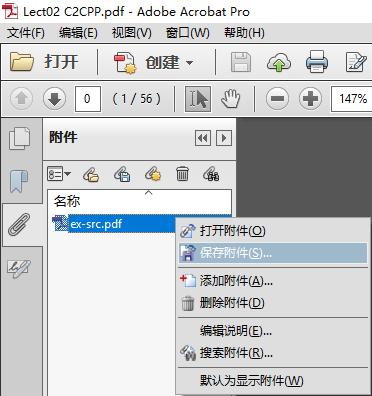
\includegraphics[height=0.35\textheight]{pdfattatchdownload01}\quad
    %或 \quad%
    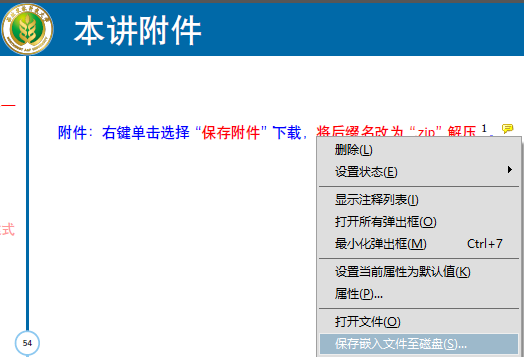
\includegraphics[height=0.35\textheight]{pdfattatchdownload02}\\[2ex]%
    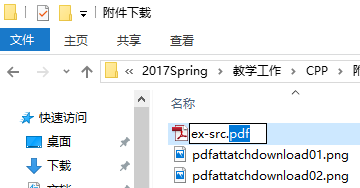
\includegraphics[height=0.255\textheight]{pdfattatchdownload03}\quad
    %$\Rightarrow$ \quad%
    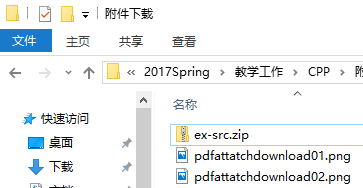
\includegraphics[height=0.255\textheight]{pdfattatchdownload04}%
  \end{center}   
\end{frame}

% \tiny
% \scriptsize
% \footnotesize
% \small
% \normalsize
% \large
% \Large
% \LARGE
% \huge
% \Huge


%%% Local Variables: 
%%% mode: latex
%%% TeX-master: "../main.tex"
%%% End: 
